\section{Cinematica del punto materiale}

Preso come riferimento il sistema di assi ($x$, $y$, $z$) le coordinate in funzione del tempo del punto $P$ che si muove avente traiettoria $s$ saranno

\begin{equation*}
    \begin{cases}
        x = x(t) \\
        y = y(t) \\
        z = z(t)
    \end{cases}
\end{equation*}

\begin{figure}[!ht]
    \centering
    \begin{tikzpicture}
        \draw[black, thin, -latex] (0,0) -- (6,0) node[anchor=north] {$y$};
        \draw[black, thin, -latex] (0,0) -- (0,4) node[anchor=east] {$z$};
        \draw[black, thin, -latex] (0,0) -- (-1,-1) node[anchor=east] {$x$};
        \filldraw[black] (0,0) circle (1pt) node[anchor=east] {$O$};

        \draw[accent, very thick] (1,2) .. controls (2,2) and (3,4) .. (4,2);
        \draw[accent, very thick] (1,2) .. controls (0,2) and (-1,3) .. (-2,1)
        node[pos=.8, anchor=south east] {$s$};

        \draw[black, very thick, -latex] (0,0) -- (1,2)
        node[pos=.5, anchor=south east] {$\vect{r}(t)$};

        \draw[black, very thick, -latex] (0,0) -- (3.66,2.5)
        node[pos=.5, anchor=north west] {$\vect{r}(t + \Delta t)$};

        \draw[accent, very thick, -latex] (1,2) -- (3.66,2.5)
        node[black, pos=.5, anchor=north] {$\Delta \vect{r}$}; % PP'

        \filldraw[black] (3.66,2.5) circle (1pt) node[anchor=south west] {$P'$};
        \filldraw[black] (1,2) circle (1pt) node[anchor=south] {$P$};
    \end{tikzpicture}
    \caption{}
\end{figure}

Il vettore avente origine in $O$ definirà lo spostamento del punto $P$ e verrà indicato con $\vect{r}$ in funzione del tempo

\begin{equation}
    \vect{OP} = x(t) \vect{i} + y(t) \vect{j} + z(t) \vect{k}
\end{equation}

Per un intervallo ($t$, $t + \Delta t$) la posizione del punto $P$ sarà quindi definita

\begin{equation}
    \vect{PP'} = \vect{r} (t + \Delta t) - \vect{r} (t) = \Delta x \vect{i}  +  \Delta y \vect{j} + \Delta z \vect{k}
\end{equation}

Per un intervallo infinitesimo, posto $d\vect{r} = \vect{PP'}$ con $\Delta t \to 0$, lo spostamento è $d \vect{r} = \vect{i} x + \vect{i} j + \vect{i} k$.

Il numero minimo di coordinate necessario per definire univocamente un sistema si chiama numero di \textcolor{accent}{gradi di libertà}.



\subsection{Moto rettilineo uniforme}

\begin{figure}[!h]
    \centering
    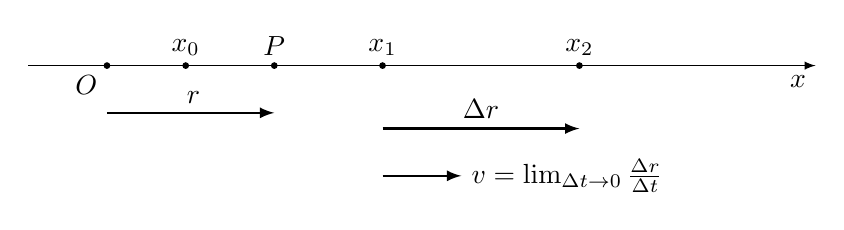
\begin{tikzpicture}
        \draw[black, thin, -latex] (-1,0) -- (9,0) node[anchor=north east] {$x$};
        \filldraw[black] (0,0) circle (1pt) node[anchor=north east] {$O$};

        \filldraw[black] (1,0) circle (1pt) node[anchor=south] {$x_0$};
        \filldraw[black] (3.5,0) circle (1pt) node[anchor=south] {$x_1$};
        \filldraw[black] (6,0) circle (1pt) node[anchor=south] {$x_2$};

        \draw[black, thick, -latex] (0,-.6) -- (2.125,-.6);
        \draw[black] (1.1,-.6) node[anchor=south] {$\vect{r}$};
        \filldraw[black] (2.125,0) circle (1pt) node[anchor=south] {$P$};

        \draw[black, thick, -latex] (3.5,-.8) -- (6,-.8);
        \draw[black] (4.75,-.8) node[anchor=south] {$\Delta \vect{r}$};
        \draw[black, thick, -latex] (3.5,-1.4) -- (4.5,-1.4) node[anchor=west] {            $\vect{v} = \lim_{\Delta t \to 0} \frac{\Delta \vect{r}}{\Delta t}$};
    \end{tikzpicture}
    \caption{}
\end{figure}

Considerato un punto materiale che si muova su una traiettoria rettilinea, posta come origine $O$ e come posizione iniziale del punto $x_0$ l'equazione oraria che descrive il moto di $P$ sarà

\begin{equation}
    x = x_0 + x(t) = x_0 + v t
\end{equation}

La \emph{velocità scalare} (media) $v$ di conseguenza avrà intensità

\begin{equation}
    v = \frac{x_2 - x_1}{t_2 - t_1}
\end{equation}

Mentre il \emph{vettore velocità} $\vect{v}$ ha direzione tangente alla traiettoria di $P$ (in questo caso l'asse $x$), verso del moto e intensità pari a $v_s$

\begin{equation}
    \vect{v} = \lim_{\Delta t \to 0} \frac{\Delta \vect{r}}{\Delta t} = \frac{d \vect{r}}{d t}
\end{equation}

\begin{equation}
    v_s = \lim_{\Delta t \to 0} \frac{x (t + \Delta t) - x(t)}{\Delta t}
\end{equation}

\begin{equation}
    \vect{v} = \frac{d \vect{r}}{dt}  = \vect{i} \frac{d x(t)}{dt}  = \vect{i} \dot{x} = \vect{i} v
\end{equation}

\begin{equation}
    \label{eq:velocità_dimensioni}
    [v] = [L T^{-1}]
\end{equation}



\subsection{Moto rettilineo vario}

\begin{figure}[!h]
    \centering
    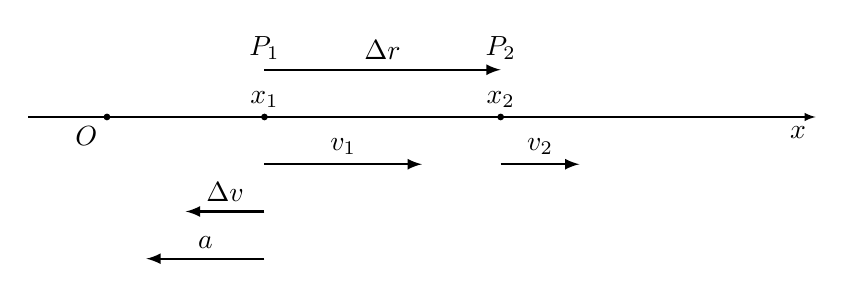
\begin{tikzpicture}
        \draw[black, thin, -latex] (-1,0) -- (9,0) node[anchor=north east] {$x$};  % x axis
        \filldraw[black] (0,0) circle (1pt) node[anchor=north east] {$O$};  % origin

        \filldraw[black] (2,0) circle (1pt) node[anchor=south] {$x_1$};     % x_1

        \filldraw[black] (5,0) circle (1pt) node[anchor=south] {$x_2$};     % x_2

        \draw[black, thick, -latex] (2,.6) -- (5,.6);                       % delta r vec
        \draw[black] (3.5,.6) node[anchor=south] {$\Delta \vect{r}$};     % delta r label

        \draw[black] (2,.6) node[anchor=south] {$P_1$};                     % P_1
        \draw[black] (5,.6) node[anchor=south] {$P_2$};                     % P_2

        \draw[black, thick, -latex] (2,-.6) -- (4,-.6);                     % v_1 vec
        \draw[black] (3,-.6) node[anchor=south] {$\vect{v}_1$};           % v_1 label

        \draw[black, thick, -latex] (5,-.6) -- (6,-.6);                     % v_2 vec
        \draw[black] (5.5,-.6) node[anchor=south] {$\vect{v}_2$};         % v_2 label

        \draw[black, thick, -latex] (2,-1.2) -- (1,-1.2);                   % delta v vec
        \draw[black] (1.5,-1.2) node[anchor=south] {$\Delta \vect{v}$};   % delta v label

        \draw[black, thick, -latex] (2,-1.8) -- (.5,-1.8);                  % a vec
        \draw[black] (1.25,-1.8) node[anchor=south] {$\vect{a}$};         % a label
    \end{tikzpicture}
    \caption{}
\end{figure}

Considerato un punto materiale in moto su una traiettoria rettilinea la sua velocità sarà definita da

\begin{equation}
    \vect{v} = \vect{v} (t) = \vect{i} \dot{x} (t) = \vect{i} v
\end{equation}

Definiti due istanti $t_1$ e $t_2$ tali che $\Delta t = t_2 - t_1$, siano $P_1$ e $P_2$ le posizioni assunte dal punto materiale rispettivamente in $t_1$ e in $t_2$ e $\vect{v}_1$ e $\vect{v}_2$ le rispettive velocità, tali che $\Delta \vect{v} = \vect{v}_2 - \vect{v}_1$ in $\Delta t$. Si definisce \textcolor{accent}{accelerazione} vettoriale

\begin{equation}
    \begin{split}
        & \highlight{\vect{a} = \lim_{\Delta t \to 0} \frac{\Delta \vect{v}}{\Delta t} = \frac{d \vect{v}}{d t}} = \frac{d^2 \vect{r}}{d t^2} = \\
        &= \vect{i} \ddot{x} (t) = \vect{i} \frac{d v_s (t)}{d t} = \vect{i} a_t
    \end{split}
\end{equation}



\subsection{Moto rettilineo uniformemente accelerato}
\begin{align*}
    a_t & = \frac{v - v_0}{t - t_0}
        &
    v   & = v_0 + a_t t \text{, con $t_0 = 0$}
\end{align*}

Considerando la velocità media $v_m$ in $(0,t)$

\begin{align*}
    v_m & = \frac{1}{t} \int_0^t v(t) dt = \frac{v_0 + v}{2} & v_m & = \frac{y - y_0}{t} & y - y_0 & = \frac{1}{2} (v_0 + v) t
\end{align*}

\begin{equation}
    \highlight{y = \int_0^t v dt =  y_0 + v_0 t + \frac{1}{2} a t^2} \text{, con $y_0$ posizione nell'istante $t_0$.}
\end{equation}



\subsection{Moto armonico}

\begin{figure}[!h]
    \begin{tikzpicture}
        \draw[black, thin, -latex] (0,-2) -- (0,2) node[anchor=west] {$x$};
        \draw[black, thin, -latex] (0,0) -- (10.5,0) node[anchor=south east] {$\omega t$};

        \draw[black, thin, loosely dashed] (0,1) -- (8,1);

        %\draw[accent, very thick] (0,1) .. controls (1.4568,1) and (2.5432,-1) .. (4,-1);
        %\draw[accent, very thick] (4,-1) .. controls (5.4568,-1) and (6.5432,1) .. (8,1);
        \draw[accent, very thick, domain=0:9.5, samples=\tikzsamples] plot (\x, {sin(pi * \x / 3 r)});
        % \draw[accent, very thick] (0,0) sin (1.5,1) cos (3,0) sin (4.5,-1) cos (6,0) sin (7.5,1);
        \filldraw[black] (0,1) circle (1pt) node[anchor=east] {$A$};

        \draw[black, thin, loosely dashed] (3,2) -- (3,-2);
        \draw[black, thin, loosely dashed] (6,2) -- (6,-2);

        \draw[black] (3,0) node[anchor=north east] {$\pi$};
        \draw[black] (6,0) node[anchor=north west] {$2 \pi$};
    \end{tikzpicture}
    \caption{}
\end{figure}

\begin{equation}
    \label{eq:moto_armonico_spostamento}
    \highlight{x = A \sin{\omega t}}
\end{equation}

\begin{equation}
    [\omega] = [T^{-1}]
\end{equation}

Dato che il periodo di $\omega$ è $2 \pi$ tra $t$ e $t + T$

\begin{equation}
    \omega = \frac{\omega (t + T) - \omega t}{T} = \frac{2 \pi}{T} = 2 \pi \nu
\end{equation}

con $\nu = 1/T$

\begin{table}[!h]
    \centering
    \begin{tabular}{r l}
        $\omega t$ & angolo di fase \\
        $\omega$   & pulsazione     \\
        $A$        & ampiezza       \\
        $\nu$      & frequenza
    \end{tabular}
\end{table}

La velocità si ottiene derivando la (\ref{eq:moto_armonico_spostamento}) che definisce lo spostamento

\begin{equation}
    \label{eq:moto_armonico_velocità}
    v = \frac{dx}{dt} = \dot{x}(t) = A \omega \cos{\omega t}
\end{equation}

Infine derivando la velocità nella (\ref{eq:moto_armonico_velocità}) si ottiene l'accelerazione

\begin{equation}
    a_t = \frac{dv}{dt} = \ddot{x}(t) = - A \omega^2 \sin{\omega t} = \omega^2 x
\end{equation}

Nel caso in cui il centro di oscillazione del moto armonico non coincida con l'origine l'equazione oraria del moto armonico sarà

\begin{equation}
    x - x_0 = A \sin{(\omega t + \varphi)}
\end{equation}

\subsection{Moto di un punto materiale con traiettoria giacente su un piano}

\begin{figure}[!h]
    \centering
    \begin{tikzpicture}
        \draw[black, thin, -latex] (0,0) -- (5,0) node[anchor=north east] {$x$};
        \draw[black, thin, -latex] (0,0) -- (0,5) node[anchor=north east] {$y$};
        \draw[black] (0,0) node[anchor= north east] {$O$};

        \draw[accent, very thick] (-1, 3) .. controls (1,5) and (1.5,3) .. (2,2);
        \draw[accent, very thick] (2, 2) .. controls (2.5,1) and (3.5,.5) .. (5,1);

        \draw[black, thick, -latex] (0,0) -- (2.4,1.42)
        node[pos=.5, anchor=north west] {$\vect{r}(t)$};

        \draw[black, thick, -latex] (0,0) -- (1.27,3.4)
        node[pos=.5, anchor=south east] {$\vect{r}(t + \Delta t)$};

        \draw[black, thick, -latex] (2.4,1.4) -- (1.27,3.4);

        \draw[accent, very thick, -latex] (2.4,1.4) -- (1.27,2.6)
        node[black, pos=.3, anchor=east] {$\vect{v} = \frac{\Delta \vect{v}}{\Delta t}$};
        \filldraw[black] (2.4,1.42) circle (1pt) node[anchor=south west] {$P$};
        \filldraw[black] (1.27,3.4) circle (1pt) node[anchor=south west] {$P_1$};
    \end{tikzpicture}
    \caption{}
\end{figure}

Preso un sistema di assi $x$, $y$ di riferimento il moto sarà descritto dal vettore spostamento

\begin{equation}
    \vect{r}(t) = \vect{i}x(t) + \vect{j}y(t)
\end{equation}

La velocità media nell'intervallo considerato, diretta lungo la corda $\overline{PP_1}$ è definita dal vettore

\begin{equation}
    \frac{\Delta \vect{r}}{\Delta t} = \frac{\vect{r}(t + \Delta t) - \vect{r}(t)}{\Delta t}
\end{equation}

Inoltre se esiste il limite

\begin{equation}
    \highlight{\lim_{\Delta t \to 0} \frac{\Delta \vect{r}}{\Delta t} = \frac{d \vect{r}}{dt} = \vect{v} (t)}
\end{equation}

esso si definisce \textcolor{accent}{velocità istantanea}.

Derivando $\vect{r}(t)$ si ha:

\begin{equation}
    \vect{v} (t) = \frac{d \vect{r}}{dt} = \vect{i} \frac{dx(t)}{dt} + \vect{j} \frac{dy(t)}{dt}
\end{equation}

L'accelerazione è definita in modo analogo

\begin{equation}
    \frac{\Delta \vect{v}}{\Delta t} = \frac{\vect{v}(t + \Delta t) - \vect{v} (t)}{\Delta t}
\end{equation}

da cui

\begin{equation}
    \highlight{\vect{a} = \lim_{\Delta t \to 0} \frac{\Delta \vect{v}}{\Delta t}}
\end{equation}

o anche

\begin{equation}
    \vect{a} = \frac{d\vect{v}}{d t} = \frac{d^2\vect{r}}{d t^2} = \vect{i} \frac{d^2 x}{dt^2} + \vect{j} \frac{d^2 y}{dt^2}
\end{equation}

\subsection{Moto circolare uniforme}


\begin{figure}[!h]
    \centering
    \begin{tikzpicture}
        \draw[black, thin, -latex] (-3,0) -- (3,0) node[anchor=north west] {$x$};
        \draw[black, thin, -latex] (0,-3) -- (0,3) node[anchor=north east] {$y$};
        \draw[black, thin] (0,0) circle (2) node[anchor=north east] {$O$};

        \draw[black, thick, -latex] (0,0) -- (1.732, 1);

        \draw[black] (1,0) arc (0:30:1) node[anchor=north west] {$\varphi$};

        \draw[accent, very thick] (2,0) arc (0:30:2);

        \filldraw[black] (1.732, 1) circle (1pt) node[anchor=south west] {$P$};

        \draw[accent] (1.931851653, 0.51763809) node[anchor=west] {$L$};
        \draw[black] (2,0) node[anchor=north west] {$O'$};
    \end{tikzpicture}
    \caption{}
\end{figure}

\begin{equation}
    s(t) = L(t)
\end{equation}

\begin{equation}
    L(t) = v t
\end{equation}

\begin{equation}
    \varphi (t) = \frac{v}{R} t
\end{equation}

\begin{equation}
    T = \frac{2 \pi R}{v}
\end{equation}

\begin{equation}
    \omega = \frac{2 \pi}{T} = \frac{v}{R}
\end{equation}

\begin{equation*}
    \dot{L}(t) = R \dot{\varphi}(t)
\end{equation*}

\begin{equation}
    \highlight{\dot{\varphi} (t) = \frac{d \varphi (t)}{dt} = \omega}
\end{equation}


La velocità angolare vettoriale è definita da:
\begin{itemize}[noitemsep]
    \setlength{\itemindent}{6em}
    \item[\emph{direzione}] normale al piano in cui giace la traiettoria
    \item[\emph{verso}] del moto ($\vect{k}$)
    \item[\emph{intensità}] $\omega = |\dot{\varphi}(t)|$
\end{itemize}
\begin{equation}
    \vect{\omega} = \dot{\varphi}(t) \vect{k}
\end{equation}


L'accelerazione nel moto circolare è centripeta, ha solo componente normale

\begin{equation}
    a = \lim_{\Delta t \to 0} \frac{\Delta v}{\Delta t} = \frac{v^2}{R} = \omega^2 R
\end{equation}



\subsection{Moto di un punto con traiettoria qualsiasi}



\subsection{Accelerazione di un moto con traiettoria giacente in un piano}



\subsection{Moti centrali con velocità areolare}

\begin{equation}
    \highlight{\frac{d\vect{S}}{dt} = \frac{1}{2} \vect{r} \times \vect{v}}
\end{equation}



\subsection{Moti di uno stesso punto materiale rispetto a sistemi di riferimento diversi}

\subsubsection{Moto di trascinamento traslatorio}

\begin{figure}[!h]
    \centering
    \begin{tikzpicture}[scale=.7]
        \draw[black, thin, -latex] (0,0) -- (7,0) node[anchor=north east] {$x$};
        \draw[black, thin, -latex] (0,0) -- (0,6) node[anchor=north east] {$y$};
        \draw[black] (0,0) node[anchor=north east] {$O$};

        \draw[black, thin, -latex] (1,1) -- (4,1) node[anchor=north east] {$x'$};
        \draw[black, thin, -latex] (1,1) -- (1,4) node[anchor=north east] {$y'$};
        \draw[black] (1,1) node[anchor=north east] {$\Omega$};

        \filldraw[black] (2,2.5) circle (1pt) node[anchor=south west] {$P$};

    \end{tikzpicture}
    \begin{tikzpicture}[scale=.7]
        \draw[black, thin, -latex] (0,0) -- (7,0) node[anchor=north east] {$x$};
        \draw[black, thin, -latex] (0,0) -- (0,6) node[anchor=north east] {$y$};
        \draw[black] (0,0) node[anchor=north east] {$O$};

        \draw[black, thin, dashed, -latex] (1,1) -- (4,1);
        \draw[black, thin, dashed, -latex] (1,1) -- (1,4);

        \draw[black, thin, -latex] (3,2) -- (6,2) node[anchor=north east] {$x'$};
        \draw[black, thin, -latex] (3,2) -- (3,5) node[anchor=north east] {$y'$};
        \draw[black] (3,2) node[anchor=north west] {$\Omega$};

        \draw[black, thick, -latex] (1,1) -- (3,2)
        node[pos=.6, anchor=north] {$\vect{v}_t \Delta t$};

        \draw[accent, thick, -latex] (2,2.5) -- (4.5,5)
        node[black, pos=.84, anchor=east] {$\Delta \vect{s}_a$};
        \draw[accent, thick, -latex] (2,2.5) -- (4,3.5);
        \draw[accent, thick, -latex] (4,3.5) -- (4.5,5)
        node[black, pos=.5,anchor=west] {$\Delta \vect{s}_r$};
        \filldraw[black] (2,2.5) circle (1pt) node[anchor=south east] {$\overline{P}$};
        \filldraw[black] (4.5,5) circle (1pt) node[anchor=south west] {$P$};
        \filldraw[black] (4,3.5) circle (1pt) node[anchor=west] {$P'$};

    \end{tikzpicture}
    \caption{}
\end{figure}

Nel \textcolor{accent}{moto traslatorio uniforme} in cui il sistema di riferimento $x'$, $y'$ si muove a velocità costante le equazioni del moto di una particella saranno
\begin{equation*}
    \Delta \vect{s}_a = \Delta \vect{s}_r + \vect{v}_t \Delta t
\end{equation*}

Con $\Delta t \to 0$
\begin{equation}
    d \vect{s}_a = d \vect{s}_r + \vect{v}_t d t
\end{equation}
\begin{equation}
    \vect{v}_a (t) = \vect{v}_r (t) + \vect{v}_t
\end{equation}
da cui
\begin{equation*}
    \vect{a}_a = \vect{a}_r
\end{equation*}

Nel caso in cui $\vect{a}_a \ne \vect{a}_r$
\begin{equation}
    \vect{v}_a (t) = \vect{v}_r (t) + \vect{v}_t (t)
\end{equation}
\begin{equation}
    \vect{a}_a (t) = \vect{a}_r (t) + \vect{a}_t (t)
\end{equation}


\subsubsection{Moto di trascinamento di semplice rotazione}

\begin{equation}
    \highlight{\vect{v}_t = \vect{\omega} \times \vect{r}}
\end{equation}

\begin{equation}
    \highlight{\vect{a}_a = \vect{a}_r + \vect{a}_t + 2 \vect{\omega} \times \vect{v}_r}
\end{equation}


\subsubsection{Moto di trascinamento qualsiasi}

Uno spostamento del sistema ($\Omega$, $x'$, $y'$, $z'$) rispetto a un sistema fisso può esprimersi come la somma di spostamento traslatorio di $\Omega$ rispetto al sistema fisso e spostamento rotatorio intorno ad un asse. Di conseguenza ogni punto $P$ si può esprimere come somma della velocità di traslazione $\vect{v}_\Omega$ e della velocità $\vect{\omega}$ intorno a un asse per $\Omega$
\begin{equation}
    \vect{v}_t = \vect{v}_\Omega + \vect{\omega} \times \Omega \vect{P}
\end{equation}

Derivando la (\theequation) si ottiene l'\emph{accelerazione di trascinamento istantanea}
\begin{align}
    \vect{v}_a (t) & = \vect{v}_r (t) + \vect{v}_t (t)                                             \\
    \vect{a}_a (t) & = \vect{a}_r (t) + \vect{a}_t (t) + 2 \vect{\omega} (t) \times \vect{v}_r (t)
\end{align}